
\chapwithtoc{Introduction}

In today's era of information explosion and constant flow of information, it becomes more time-consuming to keep track of associations and deeply understand the published content through media and online news, primarily when investing in a specific area. For instance, the investment in a company like Apple~Inc. requires acquiring and processing a wide range of available information with significant effort and dedication in studying articles and other sources. At the same time, publicly available information resources such as news articles and tools like sentiment analysis allow us to transfer real-world context into the digital environment and use it for our benefit.

Sentiment analysis, the ability to identify and evaluate the emotional charge of content, has evolved into a crucial instrument for comprehending opinions, attitudes, and the general atmosphere surrounding various topics. This work focuses on developing an application that allows users to visualize connections between companies and news articles using a knowledge graph network and the impact of news sentiment on~a company's stock price\textcolor{lightgray}{, even in real time}.

Many experiments are currently being conducted based on historical data to examine the effect of sentiment, but not on current data, despite the rather promising results on datasets. The absence of such an application motivates this thesis. An application that extracts actual data from news articles for sentiment analysis and subsequently evaluates the future impact of that sentiment on a company's stock price.

%One potential reason for the absence of such an application may be working with a constant flow of updating data, which can present a challenge to creating a functional application. Due to the valuable nature of news sources as information providers, they protect their data against similar usage, as discussed in the Licensing and Copyright Chapter. Despite the public availability of this data, legal complications may arise from potential violations of terms and conditions, as presented in the OpenAI and The New York Times dispute outlined in the [corresponding chapter].

%Another reason is that this is still an experimental technology and a speculative approach to the market. These technologies are still evolving, and there is no clear-cut approach to 100{\%} stock price prediction depending (only) on financial news. Nevertheless, published studies involving experiments suggest correlations \textcolor{lightgray}{/? affects stock price} between stock price and news data [Links to studies]. Another notable factor is the chart [1] indicating the correlation between the number of news reports about a company and its market price. Although it may be less than 100{\%} accurate in prediction, it is an exciting topic that can be very useful for examining the impact on prices and providing an overview of the situation.
 
%\begin{figure}[hb]
%\centering
%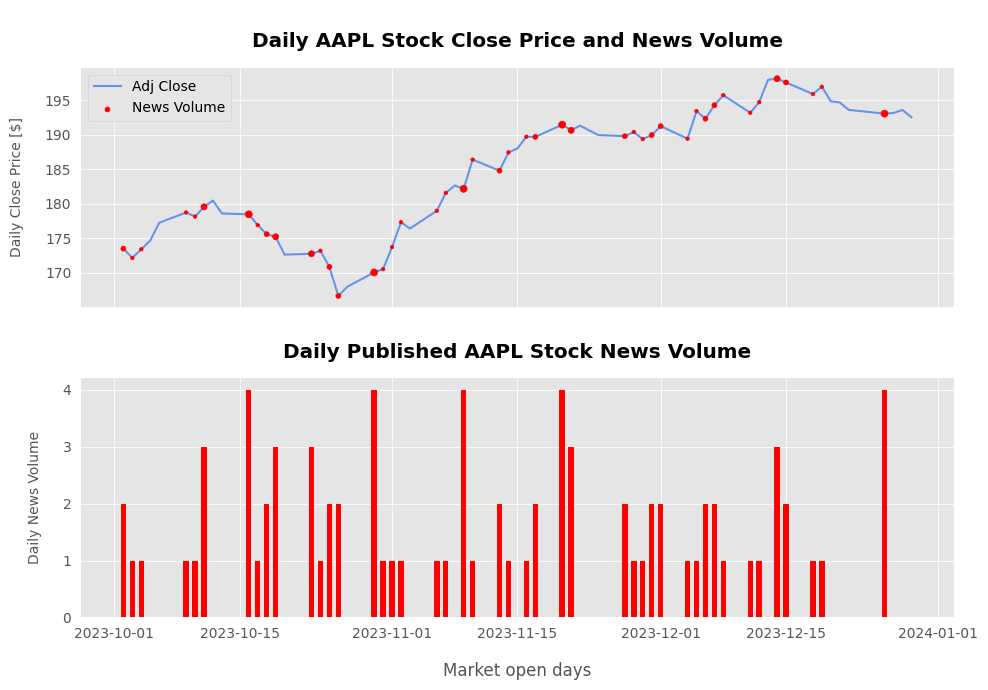
\includegraphics[width=\textwidth]{img/news_volume_impact_stock_price.pdf}
%\caption{Impact of The Guardian news on Apple Inc. stock price}
%\label{fig:f}
%\end{figure}

%\newpage
% Last paragraph of the introduction should answer the following questions:
This thesis will discuss the technical aspects of sentiment analysis and implementing an application that conveys this information to users as recently as possible. The aim is to provide users with a tool that allows them to actively monitor and analyze the flow of information about emotional overtones as one of the key identifiers in trading decisions. \textcolor{lightgray}{The thesis will be structured as follows. Chapter 1 will discuss the theoretical background behind the stock market. Chapter 2 will give an overview of data sources and the data itself. Chapter 3 will discuss the sentiment analysis and design of the application. Chapter 4 will discuss the implementation of the application. Chapter 5 will discuss the evaluation of the application. Chapter 6 will discuss the conclusion and future work.}\todo{(Q-0) Zeptat se - Jak je to s použitím 1. osoby množného čísla a pasivními formami. Tj. používání "We will, we discuss,.." a "It will be discussed, it will be implemented,..".}

